
%====|==>ICRC 2017	
\subsection{Datos presentados en la ICRC 2017}\label{icrc2015}

Se utilizaron los datos de la ICRC 2017 utilizando los cortes recomendados mencionados en la sección anterior. Además de considerar eventos con energía mayor a $1\,$EeV en un periodo de tiempo entre el 1 de Enero del 2005 y 31 de Diciembre del 2015, y con ángulo cenital $\theta$ menor que $60^o$.  Tras los cortes mencionados, se analizaron $1\,146\,470$ eventos con una media de energía de $2.00\,$EeV. Nos referiremos a este subconjunto de datos del ICRC 2017  como conjunto A. Las características de estos datos se resumen en la Tabla \ref{tabla:caracteristicas_ICRC_2017}.
%====|====|	Tabla de eventos exposure
        \begin{table}[H]
            \centering
            \begin{tabular}{r|c|} \cline{2-2}
                & ICRC 2017 \\ \cline{2-2}
            Inicio:              & 01/01/2005 \\ 
            Final:               & 31/12/2015  \\ 
            Número de eventos:   & $1\,146\,470$ \\ 
            Energía media:       & 2.00\,EeV    				\\ 
            Corte en energía:    & $> 1$ EeV        				\\ 
            Corte en ángulo cenital:		& $\theta < 60^o$ 				\\ \cline{2-2}
            \end{tabular}
        \caption{Características de los datos ICRC 2017 utilizados para el cálculo de los parámetros del clima de esta sección. } \label{tabla:caracteristicas_ICRC_2017}
        \end{table}

% ====|====|Tabla del fit
        Se realiza un ajuste de la tasa de eventos por hora del conjunto A para obtener los coeficientes promediados por ángulo cenital, que incluye todos los eventos de ángulo cenital $\theta< 60^o$. Los parámetros obtenidos se presentan y se comparan con \cite{aab2017impact} en la Tabla \ref{tabla:parametros_ICRC_2017}. Los errores presentados son los errores obtenidos por el ajuste. El $\chi^2_\nu$ representa el $\chi^2$ reducido, que para este ajuste es de $\chi^2_\nu=1.01328$, por lo que el modelo propuesto representa adecuadamente los datos experimentales. Se observa que los parámetros obtenidos son compatibles con el trabajo anterior.

        \begin{table}[H]
            \centering
            \begin{tabular}{c|c|c}
            {Parámetro}                 & {2005-2015}                   & {2005-2015}    \cite{aab2017impact}              \\ \hline \hline
            $a_P$ [hPa$^{-1}$]          & $(-3.2 \pm 0.2)\times 10^{-3}$& $(-3.2 \pm 0.3)\times 10^{-3}$    \\ \hline
            $a_\rho$ [kg$^{-1}$m$^3$]   & $-1.71 \pm 0.04 $             & $-1.72 \pm 0.04$                  \\ \hline
            $b_\rho$ [kg$^{-1}$m$^3$]   & $-0.51 \pm 0.05$              & $-0.53 \pm 0.04$                  \\ \hline
            $\chi^2_\nu$                & $1.013$                       & $1.013$                           \\ 
            \end{tabular} 
            \caption{Ajustes obtenidos considerando todos los eventos con $\theta<60^o$ y energía mayor a $1\,$EeV del conjunto del ICRC 2017, comparados con los parámetros utilizados por la Colaboración.} \label{tabla:parametros_ICRC_2017}
        \end{table}

%====|====|	2005-2016	rate hour of the day	1 EeV
        Mediante los coeficientes obtenidos se calculó la tasa de eventos por día que predice el modelo, teniendo en cuenta los valores medios de las variables del clima para cada hora. En la Fig. \ref{fig:rate_2017_05-15} se muestra el ajuste comparado con la tasa experimental. En esta figura se observa que el modelo propuesto se corresponde con los datos experimentales, como lo indica el valor de $\chi^2_\nu=1.01328$. En la Fig.\ref{fig:rate_dayly_ICRC_2017} se muestra la tasa media por día donde la modulación anual es apreciable. Mientras que en la Fig.\ref{fig:rate_hod_ICRC_2017} se muestra el promedio por cada hora del día a partir de la tasa de eventos por hora, donde la tasa medida experimentalmente presenta una modulación diaria. 
        

        \begin{figure}[H]
            \centering
            \begin{subfigure}[b]{0.875\textwidth}
            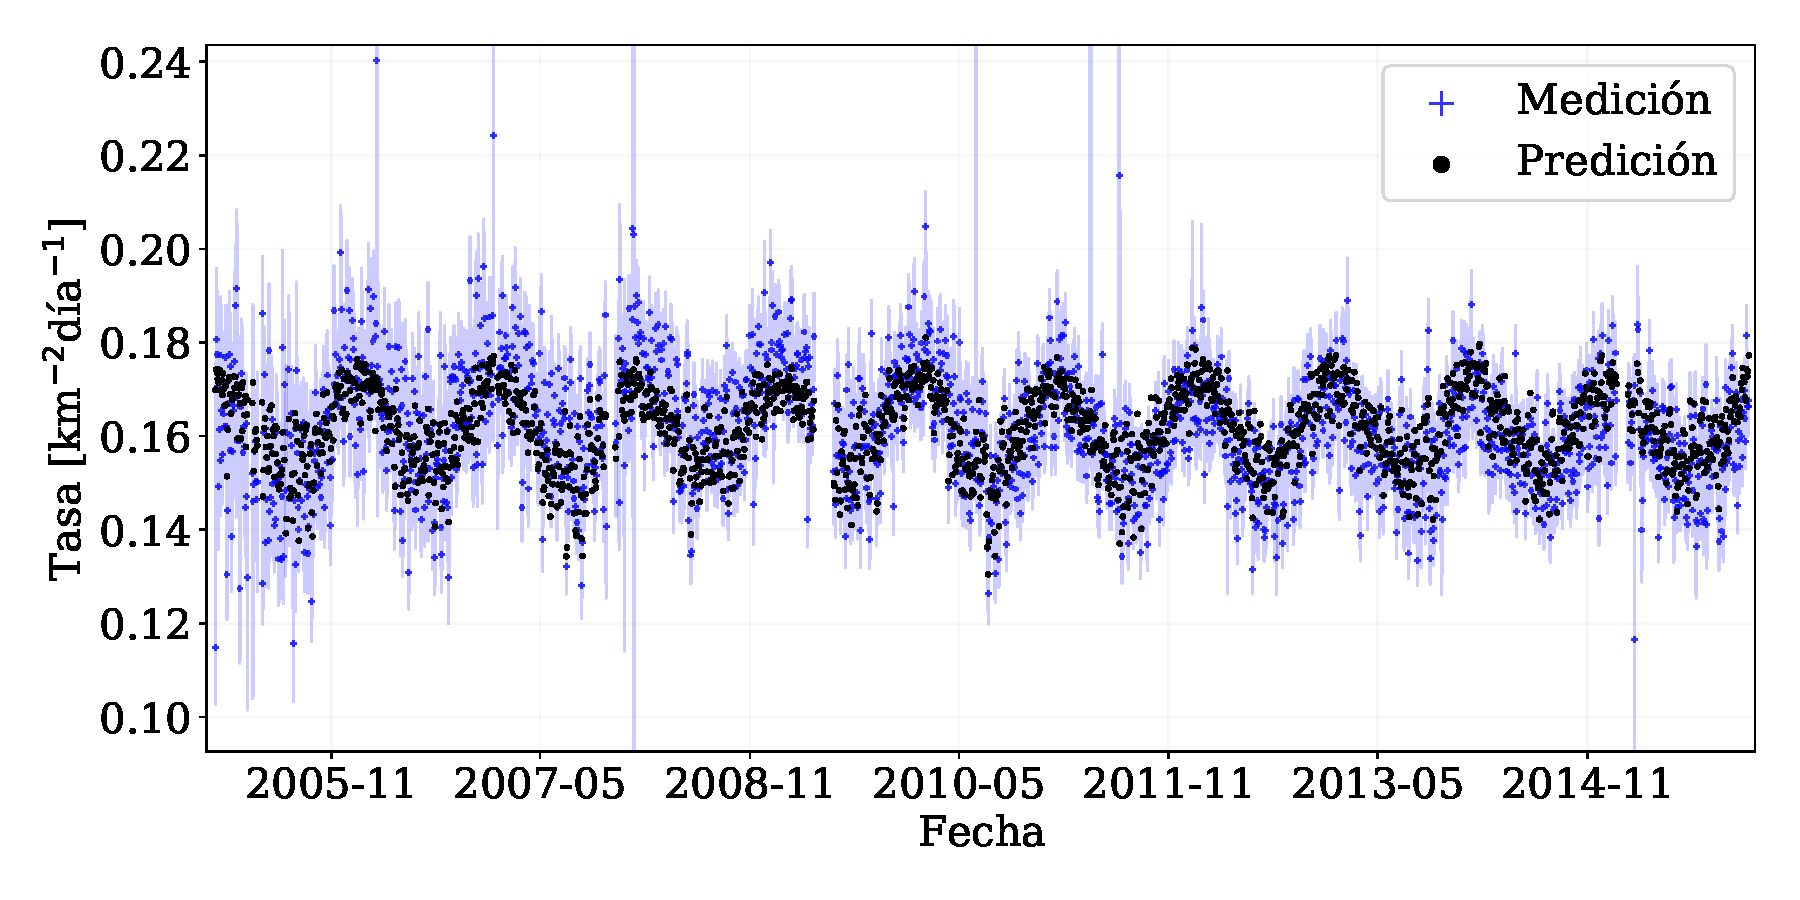
\includegraphics[width=\textwidth]{Graphs/rate_dayly/herald_old_above_1EeV_rate_day.pdf}
            \caption{Tasa eventos por día}\label{fig:rate_dayly_ICRC_2017}
            \end{subfigure}\\
            % \hspace{\fill}
            \begin{subfigure}[b]{0.875\textwidth}
            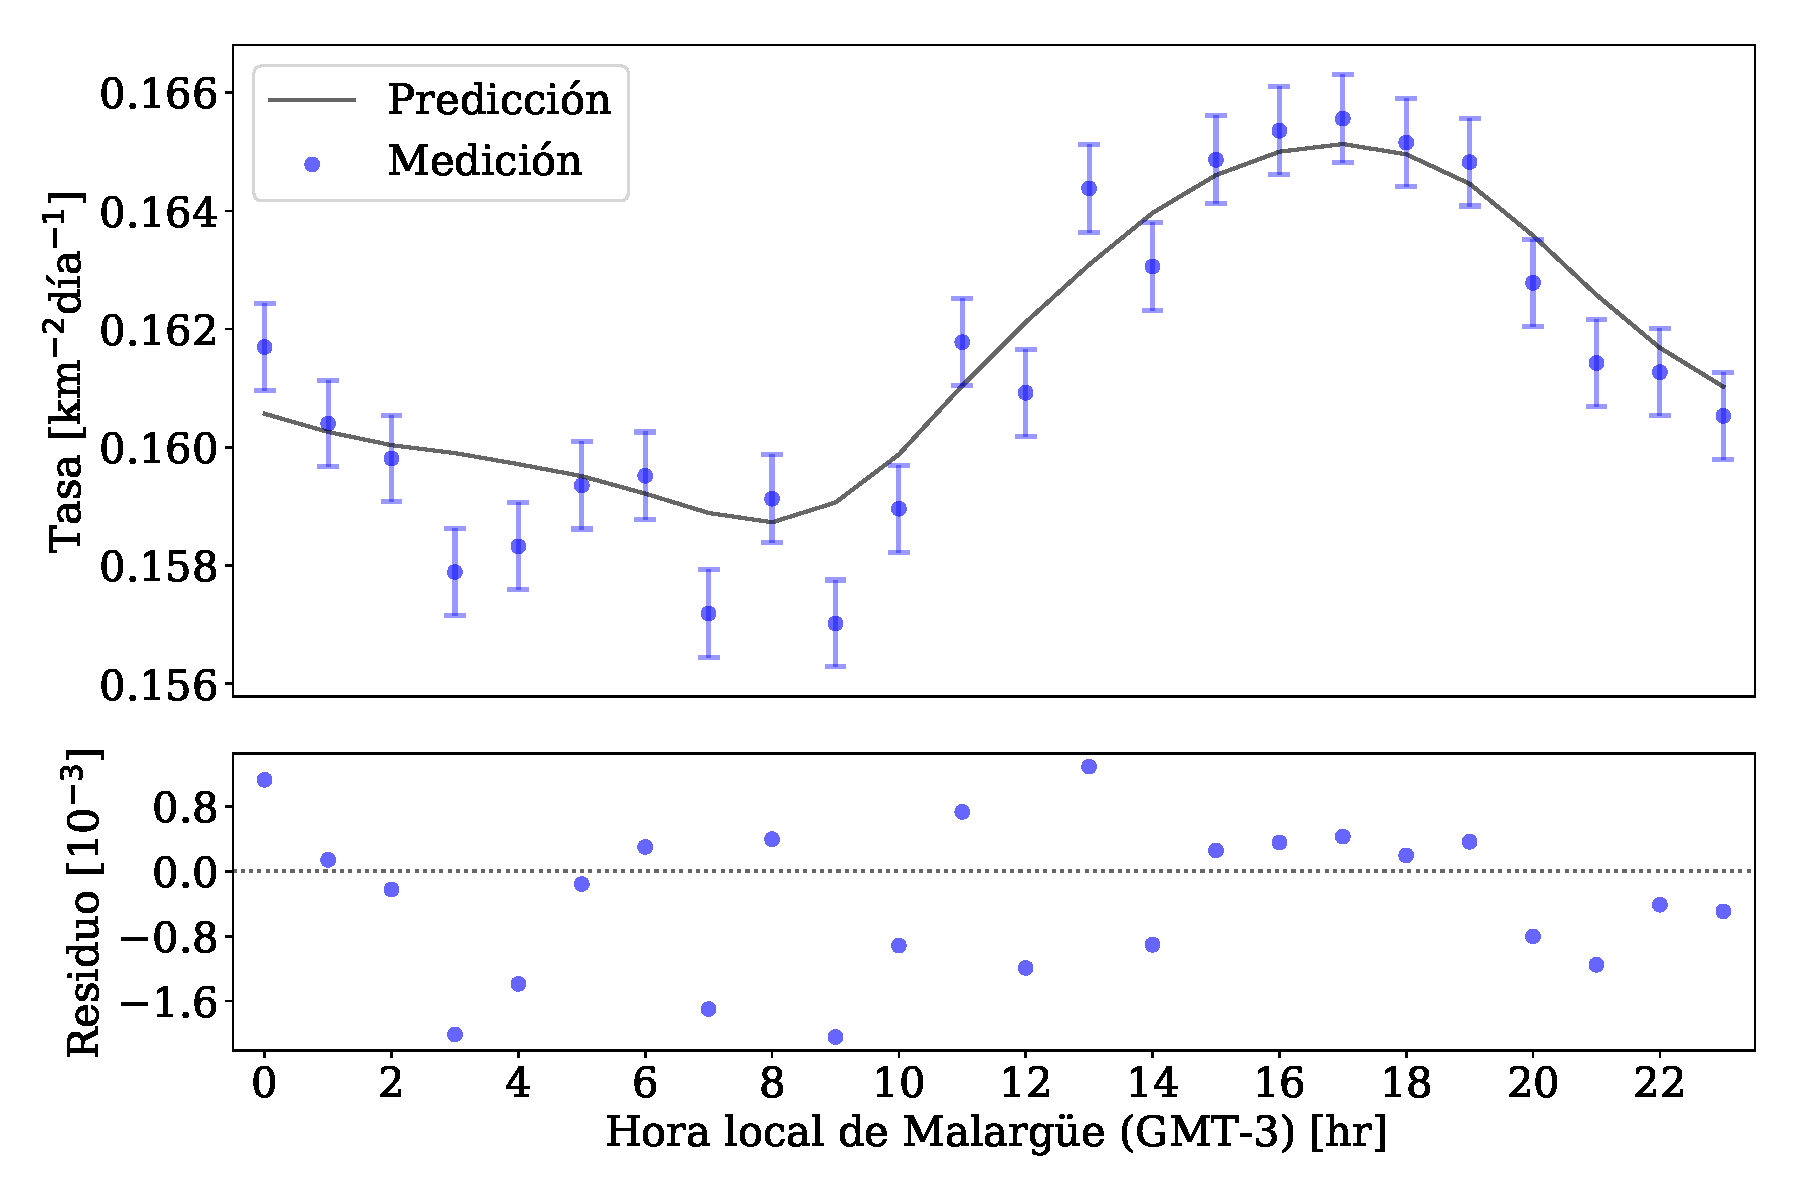
\includegraphics[width=\textwidth]{Graphs/rate_hour_of_the_day/1EeV_ICRC_2015_old_herald.pdf}
            \caption{Tasa de eventos promediada por hora del día }\label{fig:rate_hod_ICRC_2017}
            \end{subfigure}%
            \caption{Tasa de eventos por días comparadas con el ajuste entre el inicio del año 2005 hasta fines del 2015. Los datos analizados fueron los presentados en la ICRC 2017 para energías mayores a $1\,$EeV donde se observa la modulación anual y diaria del clima. }\label{fig:rate_2017_05-15}
        \end{figure}


        Como se menciona en la sección \ref{seccion:sd_eff}, el detector alcanza su máxima eficiencia para energías mayores que 3\,EeV. A partir de una energía de $2\,$EeV, los eventos tienen una mayor susceptibilidad al disparo de tres tanques, mínimo número necesario para la reconstrucción de un evento. Para el conjunto A, como se muestra en la Fig.\,\ref{fig:rate_2017_05-15_2EeV}, la modulación del clima también es apreciable para una energía mayor a $2\,$EeV con una amplitud un  poco menor que para eventos de energía mayor a $1\,$EeV. 

        \begin{figure}[H]
            \centering
            \begin{subfigure}[b]{0.875\textwidth}
            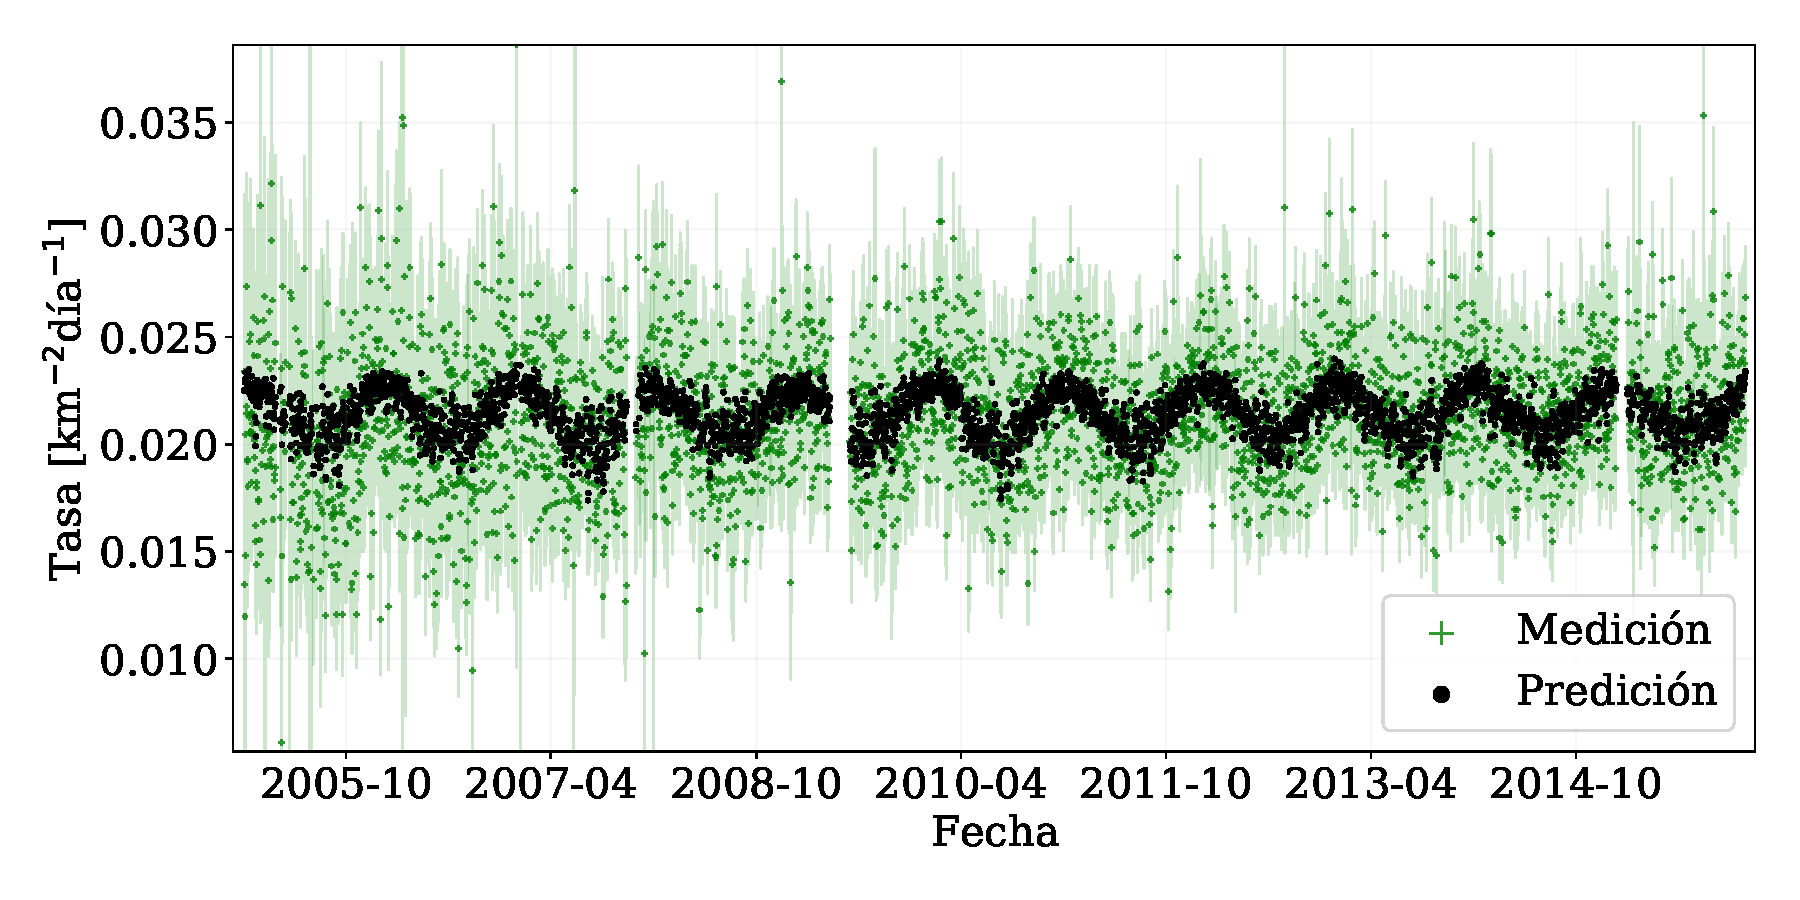
\includegraphics[width=\textwidth]{Graphs/rate_dayly/herald_old_above_2EeV_rate_day.pdf}
            \caption{Tasa eventos por día}\label{fig:rate_dayly_ICRC_2017_2EeV}
            \end{subfigure}\\
            % \hspace{\fill}
            \begin{subfigure}[b]{0.875\textwidth}
            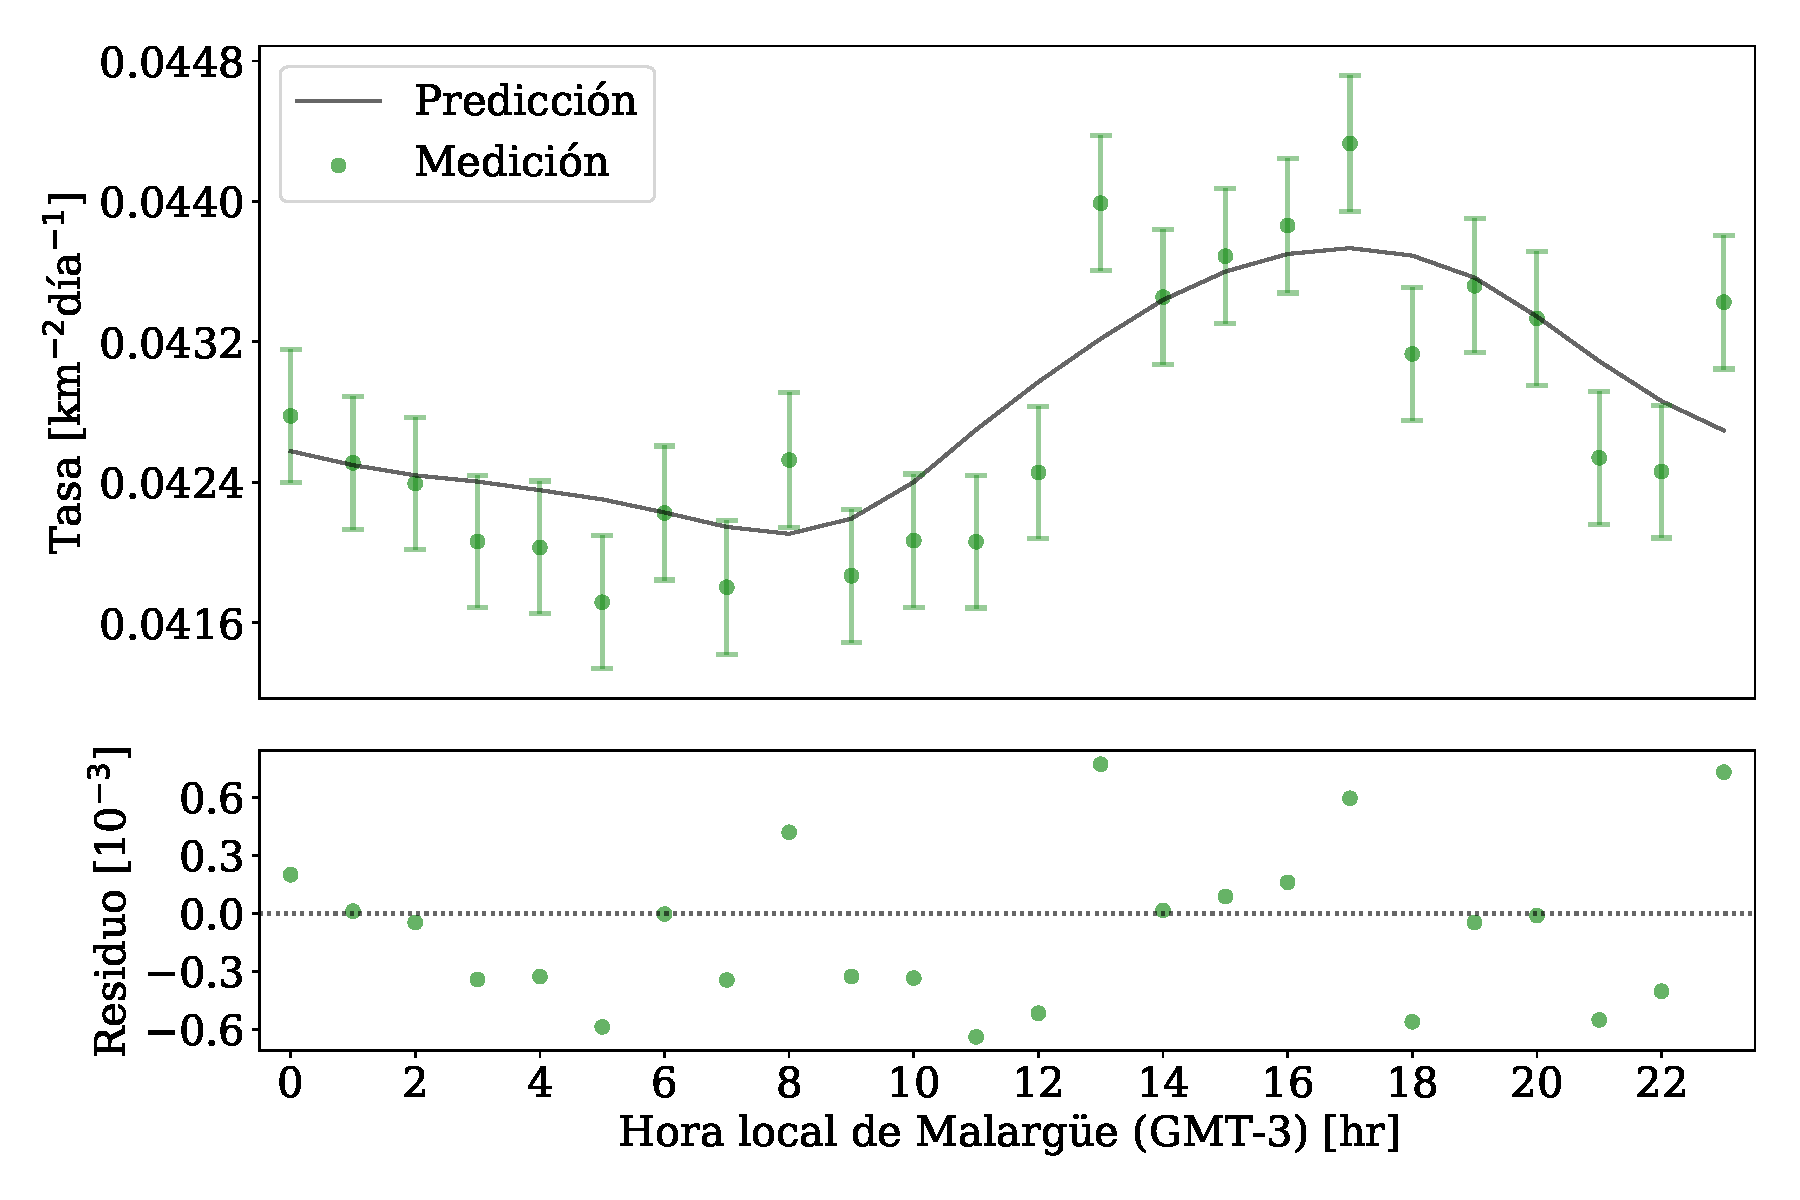
\includegraphics[width=\textwidth]{Graphs/rate_hour_of_the_day/herald_old_above_2EeV_hour_of_the_day.pdf}
            \caption{Tasa de eventos promediada por hora del día }\label{fig:rate_hod_ICRC_2017_2EeV}
            \end{subfigure}%
            \caption{Tasa de eventos por días comparadas con el ajuste entre el inicio del año 2005 hasta fines del 2015. Los datos analizados son los presentados en la ICRC 2017 para energías mayores a $2\,$EeV donde se observa la modulación anual y diaria del clima }\label{fig:rate_2017_05-15_2EeV}
        \end{figure}

%====|====|	Weather params
        \subsubsection{Ajuste de los parámetros del clima}
        En esta sección se estudia la dependencia de los parámetros del clima con el ángulo cenital. Se clasificaron los eventos en distintos grupos según el valor de $sin^2(\theta)$ para realizar un ajuste análogo al presentado en la Tabla \ref{tabla:parametros_ICRC_2017}. Se clasifica mediante este valor para obtener números de eventos similares para cada subconjunto. Estos ajustes son presentados en las Figs. \ref{fig:ap_2017}, \ref{fig:arho_2017} y \ref{fig:brho_2017}. Los mismos se comparan con los datos presentados en \cite{aab2017impact}, usados actualmente en la estimación  de la energía de los datos del Observatorio Pierre Auger. Se observa que los ajustes hechos sobre el conjunto A son compatibles con los ajustes realizados en  el trabajo \cite{aab2017impact}. 
%====|====|====|	ap, arho, brho 2005-2016 vs JINST over 1 EeV
                \begin{figure}[H]
                    \centering
                    \begin{subfigure}[b]{0.75\textwidth}
                    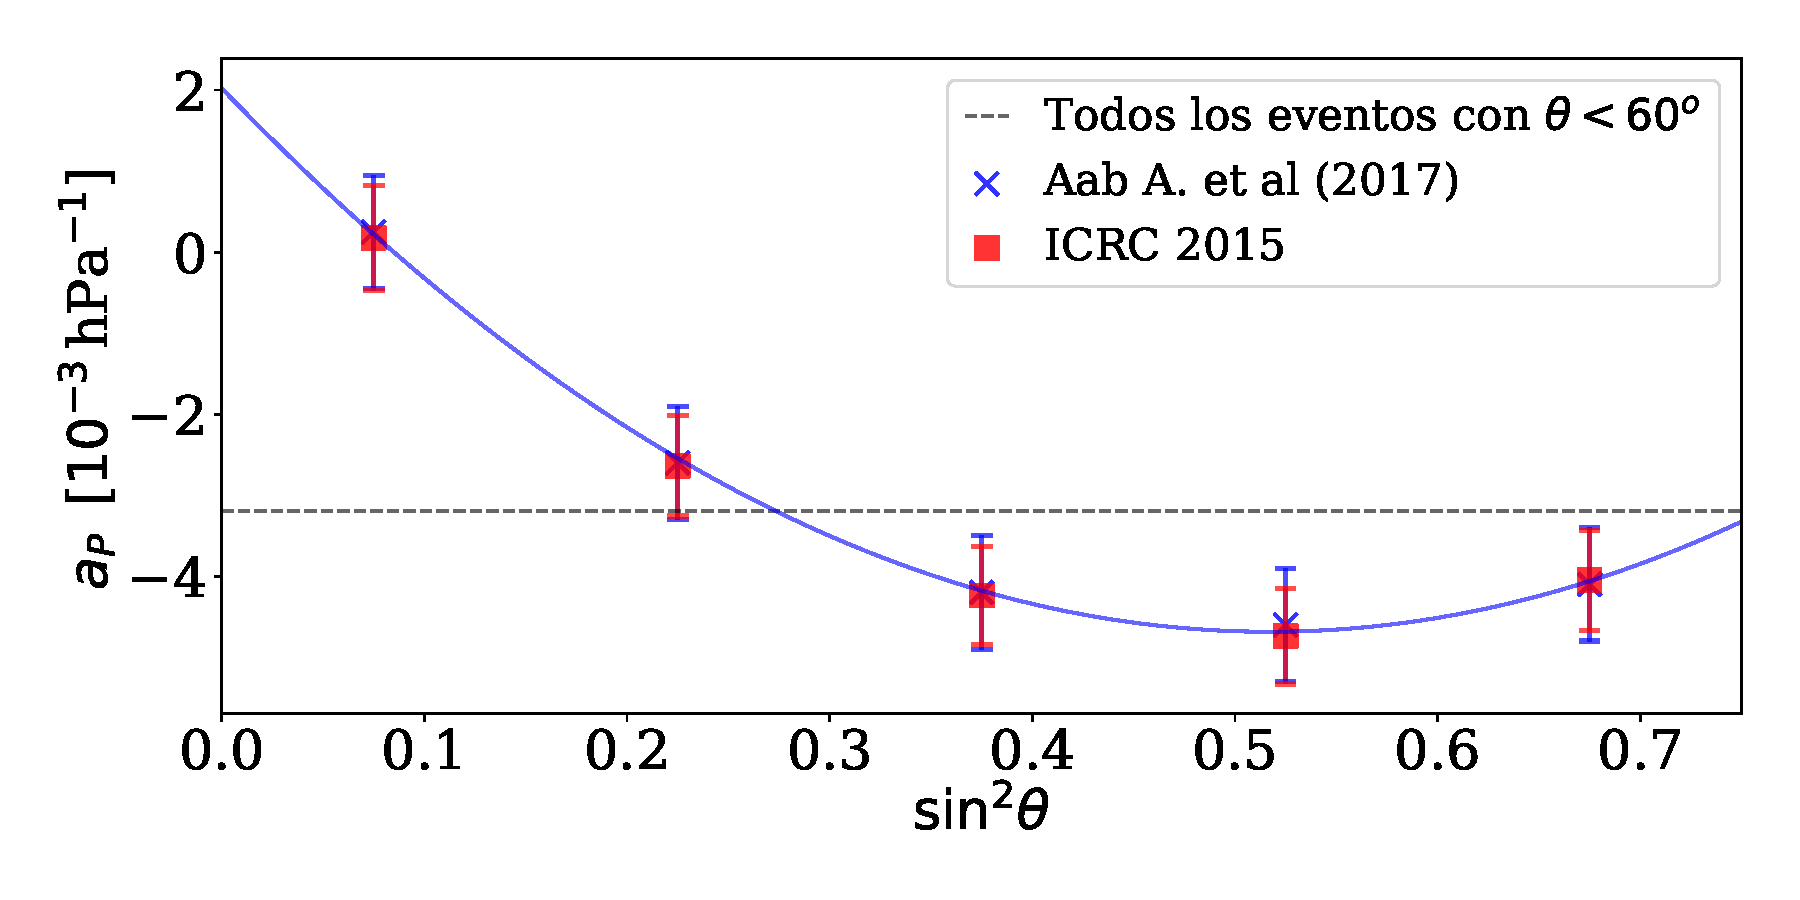
\includegraphics[width=\linewidth]{Graphs/params/ap_ICRC_2015_above_1EeV_v2.pdf}
                    \caption{Parámetro $a_P$ }
                    \label{fig:ap_2017}
                    \end{subfigure}\\
                    % \hspace{\fill}
                    \begin{subfigure}[b]{0.75\textwidth}
                    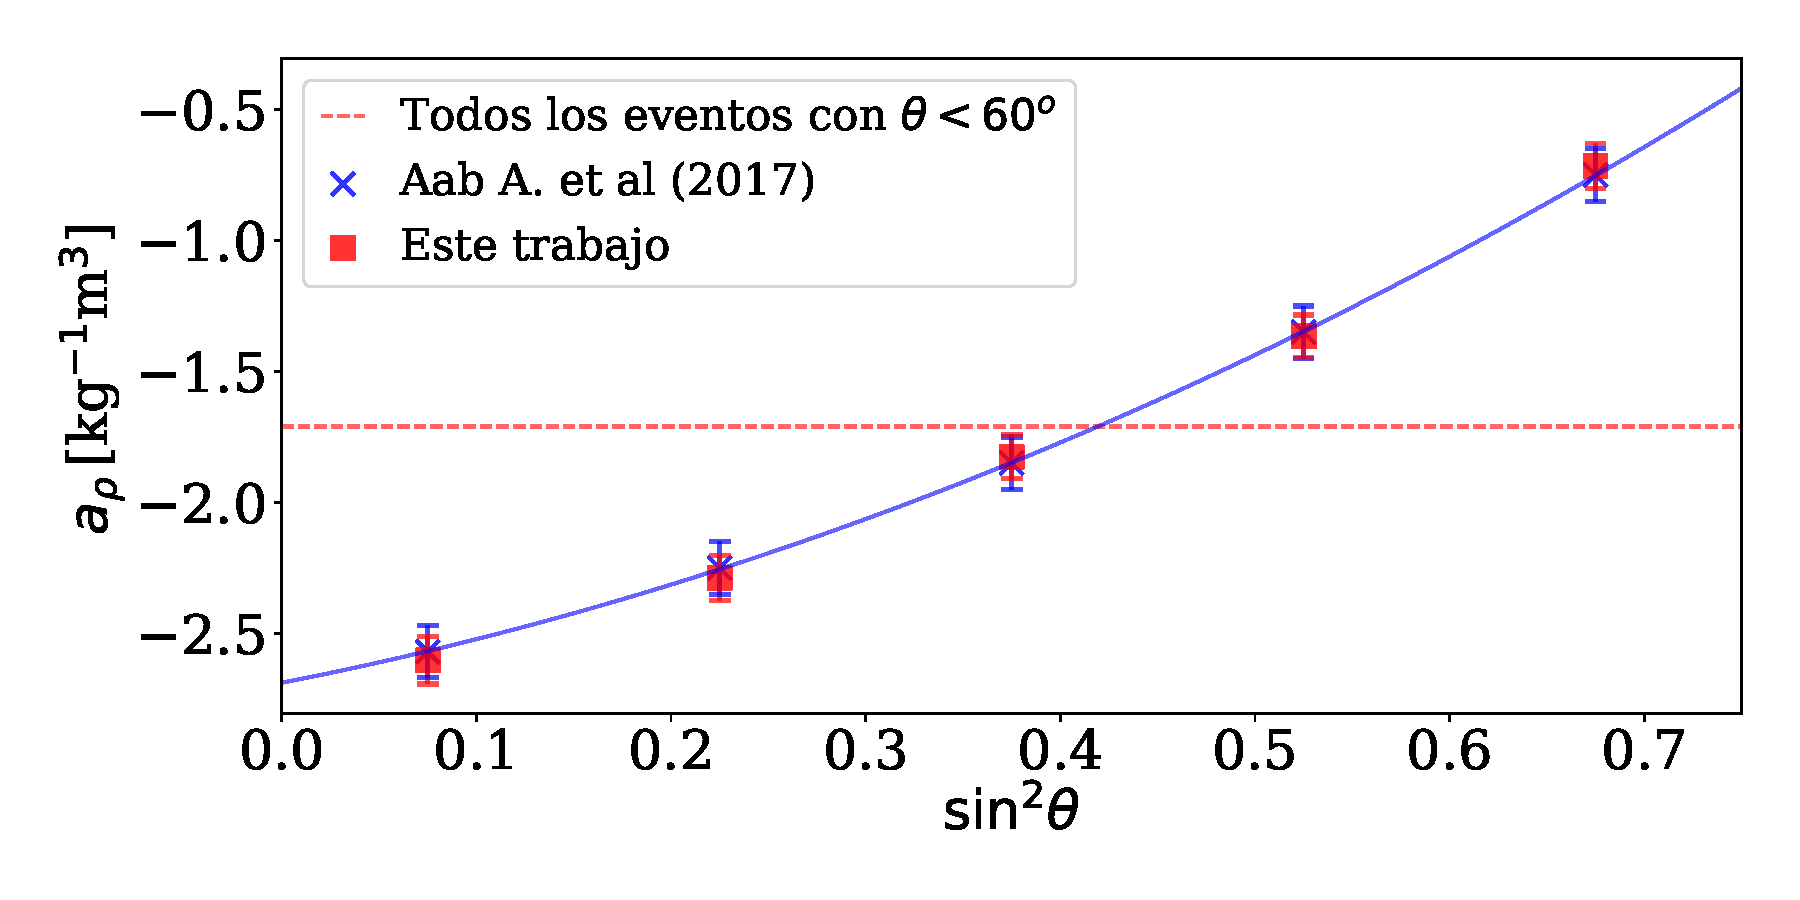
\includegraphics[width=\linewidth]{Graphs/params/arho_ICRC_2015_above_1EeV_v2.pdf}
                    \caption{Parámetro $a_{\rho}$ }
                    \label{fig:arho_2017}
                    \end{subfigure}\\
                    % \hspace{\fill}
                    \begin{subfigure}[b]{\textwidth}
                    \centering
                    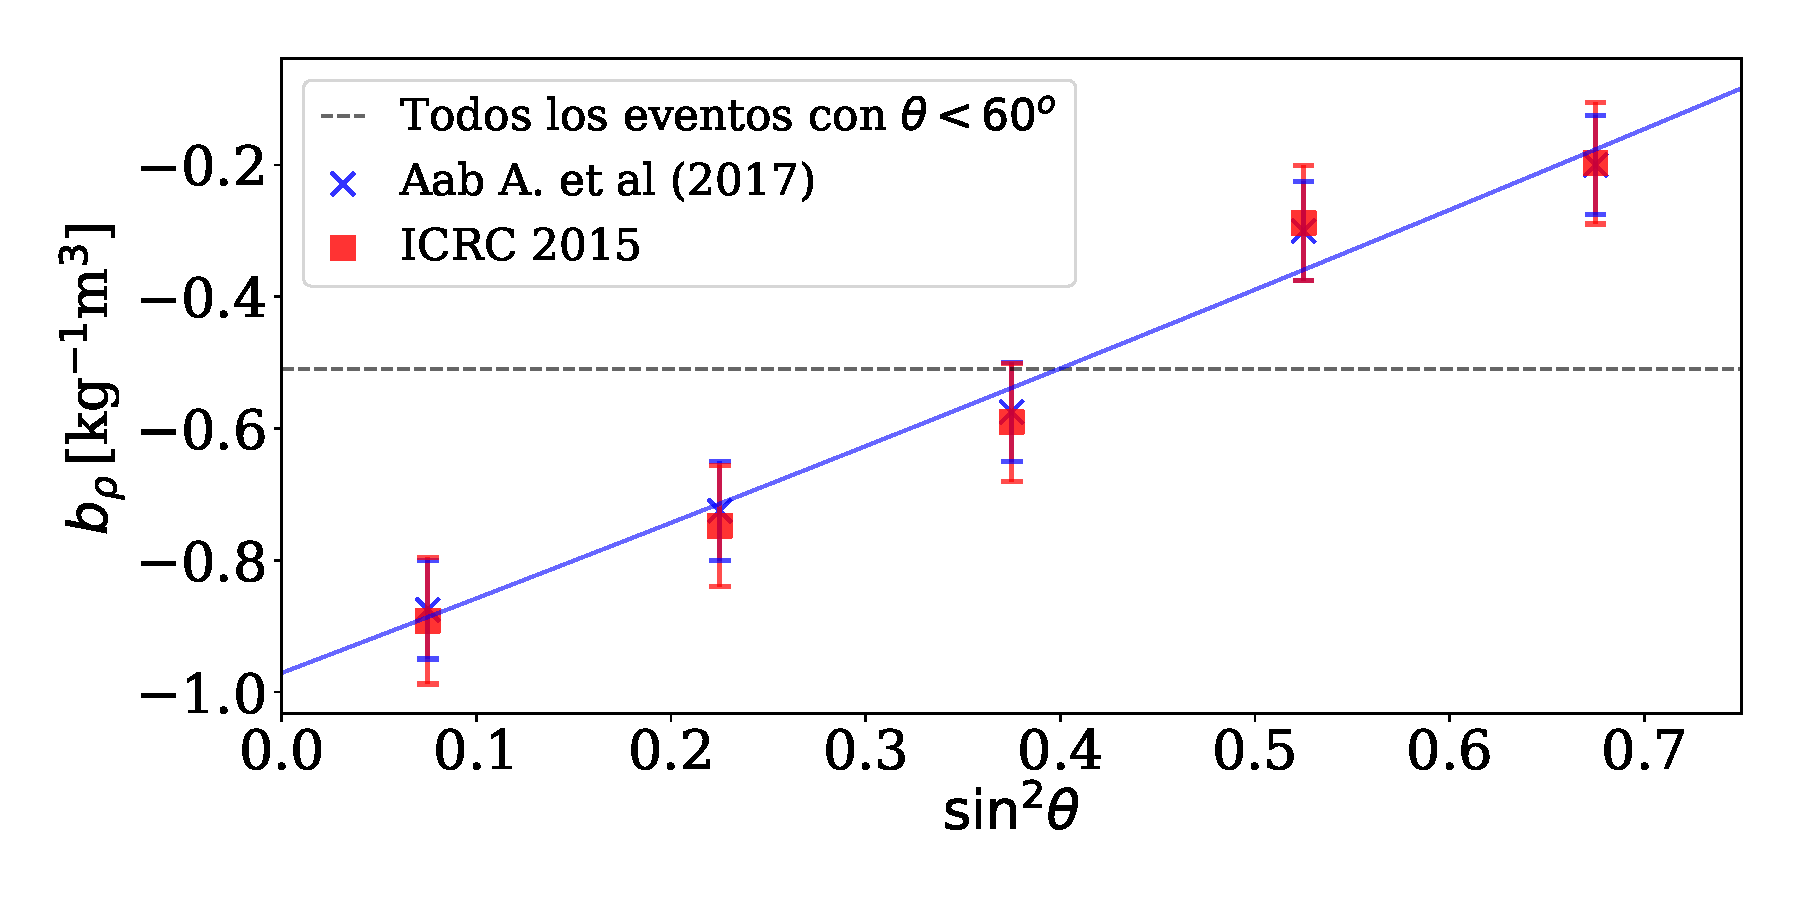
\includegraphics[width=0.75\linewidth]{Graphs/params/brho_ICRC_2015_above_1EeV_v2.pdf}
                    \caption{Parámetro  $b_{\rho}$	 }
                    \label{fig:brho_2017}
                    \end{subfigure}%
                    \caption{Parámetros de la modulación del clima considerando los datos de la ICRC 2017. Los mismos se comparan con los ajustes obtenidos por la Colaboración y con los ajustes obtenidos sin considerar la dependencia con $sin^2(\theta)$. }\label{fig:parameters_old}
                \end{figure}
%====|====|====| 	Tabla de c0, c1, c2
            En la Fig. \ref{fig:parameters_old} también se compara los ajustes obtenidos considerando los datos sin clasificar por $sin^2\theta$. Se observa que existe una dependencia con el ángulo cenital correspondiente al evento. Esta dependencia fue modelada mediante una función cuadrática dada en la Ec.\,\ref{eq:cuadratica}
            \begin{equation}
                f(x) = c_0 + c_1x + c_2x^2
                \label{eq:cuadratica}
            \end{equation}
            donde $x=sin^2\theta$.  En la Tabla\,\ref{tabla:cuadratica_ICRC_2017} se comparan los coeficientes obtenidos considerando la Ec.\,\ref{eq:cuadratica} con los mismos coeficiente obtenidos en el trabajo anterior \cite{aab2017impact}. 

        La dependencia con el ángulo cenital se debe a que para distintos ángulos de incidencia la lluvia interactúa con más o menos atmósfera. Los efectos de las condiciones climáticas afectan el desarrollo de la lluvia. Por ejemplo, el coeficiente de la presión  es negativo para $\sin^2(\theta)>0.1$ o $\theta>18^o$, lo que indica que si la presión sube la señal baja. Esto es una consecuencia de que la lluvia  está en un estado más avanzado de su desarrollo. Para ángulos cenitales cercanos a $60^o$, la componente electromagnética es suprimida por las interacciones en la atmósfera, por lo tanto el efecto de la presión disminuye. El resultado obtenido en la Fig.\,\ref{fig:ap_2017} es consistente con este fenómeno, dado que el valor de $a_P$ disminuye al aumentar el ángulo. 		En el caso de los coeficientes relacionados con la densidad, también se observa que los parámetros son negativos, dado que un aumento de la densidad disminuye $r_M$ y por lo tanto la extensión de la señal. Se observa también que los parámetros $a_\rho$ y $b_\rho$ tienen la misma tendencia con $\sin^2(\theta)$, además de que los coeficientes tienen una razón de aproximadamente $\nicefrac{1}{3}$, lo cual se esperaba por lo discutido en la sección \ref{seccion:fisica_clima}.
                \begin{table}[H]
                    \centering
                    \begin{tabular}{l|l|l|l}
                         Parámetros									& Coeficiente		& Este Trabajo			& \cite{aab2017impact}	\\ \hline \hline
                     \multirow{3}{*}{$a_P$ [hPa$^{-1}$]}  			&  $c_0$			& $( 2.00\pm 0.05)\times 10^{-3}$	& $( 2.1 \pm 0.9)\times 10^{-3} $	\\ \cline{2-4} %Done
                                                                    &  $c_1$			& $(-26.3 \pm 0.2)\times 10^{-3}$	& $(-26.0 \pm 0.6 )\times 10^{-3}$	\\ \cline{2-4} 
                                                                    &  $c_2$			& $( 25.7 \pm 0.2)\times 10^{-3}$	& $( 26.0 \pm 0.7 )\times 10^{-3}$	\\ \hline \hline% 
                    
                     \multirow{3}{*}{$a_\rho$ [kg$^{-1}$m$^3$]}  	&  $c_0$			& $-2.73   \pm 0.05$	& $ -2.7  \pm 0.1  $\\ \cline{2-4} 
                                                                    &  $c_1$			& $ 1.5    \pm 0.4 $	& $ 1.5   \pm 0.8  $\\ \cline{2-4} 
                                                                    &  $c_2$			& $ 2.1    \pm 0.7 $	& $ 2.2   \pm 1.0  $\\ \hline \hline%
                    
                    \multirow{3}{*}{$b_\rho$ [kg$^{-1}$m$^3$]} 		&  $c_0$			& $-1.0    \pm 0.1$		& $-1.0   \pm 0.1 $	\\ \cline{2-4} 
                                                                    &  $c_1$			& $ 1.2    \pm 0.6$		& $ 1.2   \pm 0.8  $	\\ \cline{2-4} 
                                                                    &  $c_2$			& $ 0.1    \pm 0.8$		& $ 0.0   \pm 1.1  $	\\ 
                    
                    \end{tabular}	
                    \caption{Tabla de los coeficientes obtenidos para el conjunto de datos de la ICRC 2017, comparados con los parámetros de la reconstrucción de los eventos del Observatorio.} \label{tabla:cuadratica_ICRC_2017}
                \end{table}

%==================================================================================
%==================================================================================
%==================================================================================
%==================================================================================

